\documentclass[10pt]{article}
\usepackage[accepted,preprint]{tmlr}
\usepackage{amsmath,amssymb}
\usepackage{booktabs}
\usepackage{graphicx}
\usepackage{hyperref}
\usepackage{url}
\hypersetup{hidelinks}

\def\month{09}
\def\year{2026}

\title{What Does a Benign-Trained Anomaly Detector Actually Detect?}

\author{\name Suramya Angdembay \email suramya.angdembay@usm.edu \\
\addr University of Southern Mississippi
\AND
\name Haiyan Tian \email haiyan.tian@usm.edu \\
\addr University of Southern Mississippi}

\begin{document}
\maketitle

\begin{abstract}
Anomaly detectors for insider threats are usually judged by how well
their scores rank malicious activity above normal activity. We show that
this number can be misleading, because it does not reveal what
information the detector uses. We build a detector by adapting a large
language model to normal employee activity only, so that unusual
activity receives a high surprisal score, and we then open the model to
determine what its score is based on. On one standard benchmark the evidence the audit selects turns out to be
almost entirely a description of who each user is (their recorded
personality and organizational profile) rather than of what they did; on a
second benchmark it is mostly behavior. When
malicious users are compared only against normal users that the model
has never seen, apparent ranking quality falls from about $0.95$ to near
chance on the first benchmark. The same analysis on a third dataset,
collected from real people with real personality questionnaires,
confirms the behavioral case, and classical statistical detectors
trained on the same information do not take the profile shortcut. Retraining the detector on text with the profile removed shows that, for
the large model we audited, the profile is the cause and not a bystander:
removal restores ranking of unseen users from chance to about $0.90$; for a
smaller model the same removal makes little measurable difference, a
contrast between two particular models that our design does not attribute
to size alone. On a corporate login log with no profile of any kind, the
same failure appears and the shortcut moves to the computer names, which
are associated with users without being fixed per user. The conclusion is that high
ranking performance alone does not show that a detector has learned to
detect behavior, and we provide a way to check.
\end{abstract}

\section{The problem}

Organizations record what employees do on their computers: logons, file
transfers, web activity, e-mail volume, and so on. An \emph{insider
threat} is an employee who misuses legitimate access, for example by
stealing data. Because such events are rare, a common approach is
\emph{anomaly detection}: build a statistical model of normal activity,
and flag days that the model finds unusual.

Formally, a detector is a function $s$ that assigns a real-valued
\emph{anomaly score} $s(x)$ to each observation $x$, where in our setting
$x$ is a record of one user's activity on one day. Higher scores are
meant to indicate more suspicious activity. Detectors are usually
evaluated by how well their scores \emph{rank} malicious days above
benign ones. The standard summary of ranking quality is the following
probability, estimated over a labeled test set:
\begin{equation}
\mathrm{AUC} \;=\; \Pr\bigl( s(X_{\mathrm{mal}}) > s(X_{\mathrm{ben}})
\bigr) \;+\; \tfrac{1}{2}\,\Pr\bigl( s(X_{\mathrm{mal}}) = s(X_{\mathrm{ben}})
\bigr),
\end{equation}
where the second term counts tied scores as half a success,
$X_{\mathrm{mal}}$ is a randomly chosen malicious day and
$X_{\mathrm{ben}}$ a randomly chosen benign day. (This quantity is
commonly called the ROC-AUC, for ``area under the receiver operating
characteristic curve''; the probability formulation above is equivalent
and is the only form we need.) An AUC of $1$ means perfect ranking and
$0.5$ means the ranking is no better than chance.

The question that motivates our work is simple to state. A high AUC says
that the score \emph{separates} the two classes. It does not say
\emph{on the basis of what information} the separation is achieved. Two
detectors with identical AUC could work very differently: one might
respond to genuinely unusual behavior, while the other might respond to
incidental properties of \emph{who} the malicious users happen to be,
such as their role, department, or personality profile. The second kind
of detector would be nearly useless in practice, because in deployment
the malicious users are not known in advance. Our paper develops a
method for determining which kind of detector one actually has, and
applies it to a modern detector built from a large language model.

\section{The data}

We use two versions (called r4.2 and r6.2) of the CERT insider-threat
corpus, a widely used synthetic dataset that simulates a corporation's
activity logs, produced by Carnegie Mellon University. Each version
contains several thousand simulated employees observed over about
eighteen months, with a small set of employees scripted to carry out
malicious scenarios on particular days. Version r4.2 has sixty malicious
users; version r6.2 has four. We later add two real datasets: TWOS, collected from real people with
real personality questionnaires, and a corporate login log with no profile
of any kind; both are described in Section~\ref{sec:findings}.

Each user-day is converted into a short structured text with three kinds
of lines:
\begin{itemize}
\item a \texttt{DAY} line holding static organizational fields for that
user (project, role, business unit, department, team, and an
information-technology administrator flag);
\item a \texttt{PSY} line holding the user's five simulated personality
scores. These are the ``Big Five'' personality traits used in
psychology: openness (O), conscientiousness (C), extraversion (E),
agreeableness (A), and neuroticism (N). In CERT these numbers are
generated by the simulator; they are constant for each user;
\item one \texttt{SES} line per work session, holding numeric behavioral
counts for that session: duration, number of logons, file and
removable-drive activity, e-mail volume, web-browsing category counts,
and similar quantities.
\end{itemize}
A user-day text therefore looks like a small table serialized as text.
The first two lines describe \emph{who the user is} and are essentially
constant across a user's days; the remaining lines describe \emph{what
the user did} that day.

\section{The detector}

\subsection{Language models as probability distributions}

A \emph{language model} is a parametric probability distribution over
sequences of symbols called tokens. Writing a sequence as
$x = (x_1, \dots, x_n)$, the model has the product form
\begin{equation}
p_\theta(x) \;=\; \prod_{t=1}^{n} p_\theta\bigl(x_t \mid x_1, \dots,
x_{t-1}\bigr),
\end{equation}
where each conditional distribution is computed by a neural network with
parameters $\theta$. Modern ``large'' language models are such networks
with billions of parameters, trained on enormous general text corpora.
We use one called Qwen3-8B (eight billion parameters). The network
processes a sequence through $L$ successive layers; at layer $\ell$ and
position $t$ it maintains an internal state vector
$h^{(\ell)}_t \in \mathbb{R}^{d}$ with $d = 4096$. These internal
vectors matter later: they are the objects we will analyze.

\subsection{Adapting the model to normal behavior only}

We specialize the general-purpose model to our corpus by
\emph{fine-tuning}: continuing its training on the serialized user-day
texts, using only days from benign users. The training objective is
maximum likelihood, that is, minimizing the negative log-likelihood of
the benign corpus $\mathcal{D}$:
\begin{equation}
\mathcal{L}(\theta) \;=\; -\sum_{x \in \mathcal{D}} \sum_{t}
\log p_\theta\bigl(x_t \mid x_{<t}\bigr).
\end{equation}
No malicious example is ever used in training. This is the classical
one-class setup: model the normal population, then measure deviation
from it.

For efficiency the fine-tuning does not modify all eight billion
parameters. Each weight matrix $W$ of the network is kept fixed and
receives a trainable low-rank correction,
\begin{equation}
W' \;=\; W + \tfrac{\alpha}{r} BA, \qquad B \in \mathbb{R}^{d_{\mathrm{out}}
\times r},\; A \in \mathbb{R}^{r \times d_{\mathrm{in}}},
\end{equation}
with rank $r = 16$, so only the small matrices $A$ and $B$ are learned.
This technique is called LoRA (low-rank adaptation); we use a
memory-saving variant called QLoRA in which the fixed weights are stored
at reduced numerical precision. The pair (fixed base model, learned
low-rank correction) is called the \emph{adapted model}. The important
point is that the entire effect of training is carried by a
low-dimensional, removable perturbation, which makes ``before versus
after'' comparisons clean.

\subsection{The anomaly score}

The score of a day $x$ is its average surprisal under the adapted
model:
\begin{equation}
s(x) \;=\; -\frac{1}{n}\sum_{t=1}^{n} \log
p_{\theta_{\mathrm{ada}}}\bigl(x_t \mid x_{<t}\bigr).
\end{equation}
Days that the model of normal behavior finds improbable receive high
scores. On the standard evaluation protocol for these benchmarks the
score ranks very well: AUC about $0.95$ on r6.2 and $0.96$ on r4.2. By
the usual standards of the field, this would be reported as a strong
detector. The rest of this document asks what that number is actually
made of.

\section{Looking inside the model}
\label{sec:plain-inside}

\subsection{What did fine-tuning change?}

Because the base model is kept frozen, we can run the same day $x$
through both the base and adapted models and subtract their internal
states. Define, at a chosen layer $\ell$ and each token position $t$,
\begin{equation}
\delta_t \;=\; h^{(\ell), \mathrm{ada}}_t - h^{(\ell),
\mathrm{base}}_t \;\in\; \mathbb{R}^{d}.
\end{equation}
The vector $\delta_t$ isolates the representational change induced by
the fine-tuning at the audited layer and position. It is the natural
object to study if one wants to know what the adaptation, as opposed to
the general-purpose model, contributes at that point in the
computation.

\subsection{A sparse dictionary for the changes}

The vectors $\delta_t$ live in $\mathbb{R}^{4096}$ and are not
individually interpretable. We therefore approximate them by sparse
nonnegative combinations of learned dictionary elements. Concretely, we
seek a dictionary matrix $D \in \mathbb{R}^{d \times m}$ (with $m = 4d$
columns, called \emph{features}) and, for each $\delta_t$, a coefficient
vector $z_t \in \mathbb{R}^{m}_{\geq 0}$ with at most $k = 8$ nonzero
entries, such that
\begin{equation}
\delta_t \;\approx\; D z_t ,
\end{equation}
with $D$ and the code map chosen to minimize the mean squared
reconstruction error over a large sample of token positions. This is a
sparse coding problem; in the machine-learning literature the particular
parametrization we use (a one-layer encoder network followed by a
keep-the-largest-$k$ rule and a linear decoder) is called a \emph{sparse
autoencoder}. The outcome is that each change vector is expressed as a
short combination of reusable directions, and each direction can be
studied on its own.

\subsection{Selecting candidate features}

Some dictionary features activate similarly on malicious and benign
days; those cannot carry the anomaly signal. We rank features by the
difference in mean activation,
\begin{equation}
g_f \;=\; \mathbb{E}\bigl[z_{t,f} \mid \text{malicious day}\bigr] -
\mathbb{E}\bigl[z_{t,f} \mid \text{benign day}\bigr],
\end{equation}
and take the five features with the largest $g_f$ as the candidate
mechanism. The full paper verifies, through intervention experiments,
that these selected features genuinely influence the anomaly score: if
one edits the coefficients $z_{t,f}$ of the selected features and
propagates the edited internal state through the rest of the network,
the score changes, and it changes more than when the same edit is
applied to matched control features. We omit the details of those
experiments here and take away only their conclusion: the selected
features are causally connected to the score, not merely correlated
with it. Figure~\ref{fig:effects} summarizes those measurements.

\begin{figure}[t]
\centering
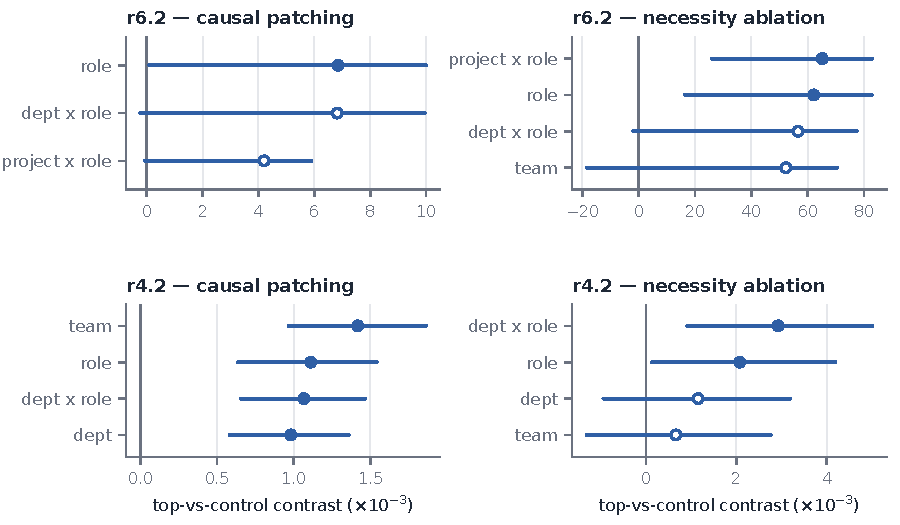
\includegraphics[width=\textwidth]{figures/mech_effects.pdf}
\caption{Effect of editing the selected features, compared with editing
matched control features, on the anomaly score (one panel per benchmark
and per type of edit; units are thousandths of the score). Each point is
the average effect for one organizational matching context, and each
horizontal bar is a $95$ percent confidence interval computed with the
malicious users as the resampling unit. Positive values mean that the
selected features influence the score more strongly than the control
features do. Open circles mark intervals that include zero.}
\label{fig:effects}
\end{figure}

\subsection{Reading off what the features respond to}

Finally we ask \emph{where} the selected features activate within the
day text. Every token position belongs to one line class: the
organizational \texttt{DAY} line, the personality \texttt{PSY} line, or
a behavioral \texttt{SES} line. For a feature $f$, define its
\emph{attribution mass} on class $c$ as the fraction of its total
activation that occurs at positions of that class:
\begin{equation}
m_f(c) \;=\;
\frac{\sum_{(x,t)\,:\, \mathrm{class}(t) = c} z_{t,f}(x)}
     {\sum_{(x,t)} z_{t,f}(x)} .
\end{equation}
If a feature has nearly all of its mass on \texttt{PSY} and \texttt{DAY}
positions, it responds to who the user is; if its mass lies on
\texttt{SES} positions, it responds to what the user did. This single
quantity is what turns the analysis into an answer to our opening
question.

\section{Findings}
\label{sec:findings}

\subsection{Two detectors that look alike and are not}

The two CERT versions produce nearly identical headline AUC values, yet
the analysis above reveals qualitatively different detectors.

On r6.2, the five selected features place between $99.8$ and $100$
percent of their attribution mass on the personality and organizational
lines. The evidence the audit selects, the five features that most raise the
score, is almost entirely a description of \emph{who the user is}. On r4.2, four of the five
selected features concentrate on the behavioral session lines. There,
the evidence is mostly \emph{what the user did}.
Figure~\ref{fig:attribution} summarizes this contrast, together with
the real-data result of Section~\ref{sec:plain-twos}.

\begin{figure}[t]
\centering
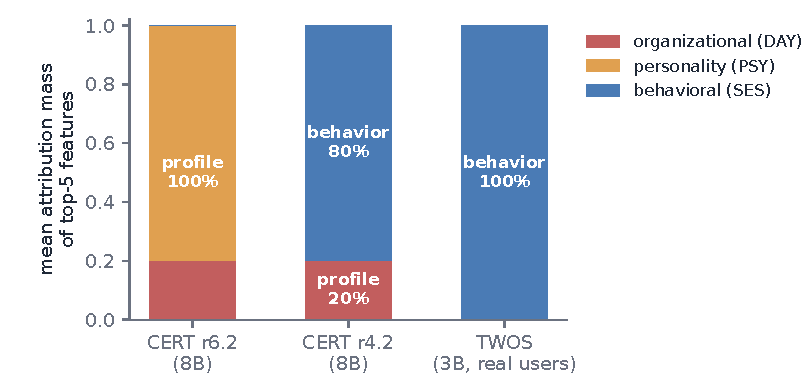
\includegraphics[width=0.85\textwidth]{figures/attribution_summary.pdf}
\caption{Where the selected features place their activation, averaged
over each detector's five selected features. Each bar decomposes the
activation mass into the organizational lines, the personality lines,
and the behavioral session lines of the input text. The r6.2 detector's selected features respond almost entirely to who the
user is; the r4.2 and TWOS detectors' selected features respond almost
entirely to what the user did.}
\label{fig:attribution}
\end{figure}

\subsection{The consequence for the headline numbers}

Why would reading a user's static profile produce a high AUC at all? The
adapted model was trained on roughly ninety percent of the benign users.
For those users, the model has been repeatedly exposed to the constant
profile lines, so their profile text is comparatively familiar and their
days look unsurprising. The malicious users, however, were never
seen in training, so their profile lines alone make their days look
surprising. The score is then partly measuring \emph{familiarity} rather
than behavior.

This suggests a sharper test: compare malicious days only against benign
days of users who were also excluded from training, so that both sides
are equally unfamiliar. Under this comparison the AUC falls from $0.95$
to $0.55$ on r6.2, which is barely better than chance, and from $0.96$
to $0.67$ on r4.2. The apparently excellent detector on r6.2 was, to a
first approximation, an unfamiliar-user detector. Consistently with
this, deleting the personality lines from the inputs at scoring time
\emph{improves} the r4.2 detector's performance on unseen users from
$0.67$ to about $0.80$: the profile text was not merely unhelpful, it
was actively obscuring the behavioral signal. Figure~\ref{fig:collapse}
shows the comparison with standard detectors and the collapse.

\begin{figure}[t]
\centering
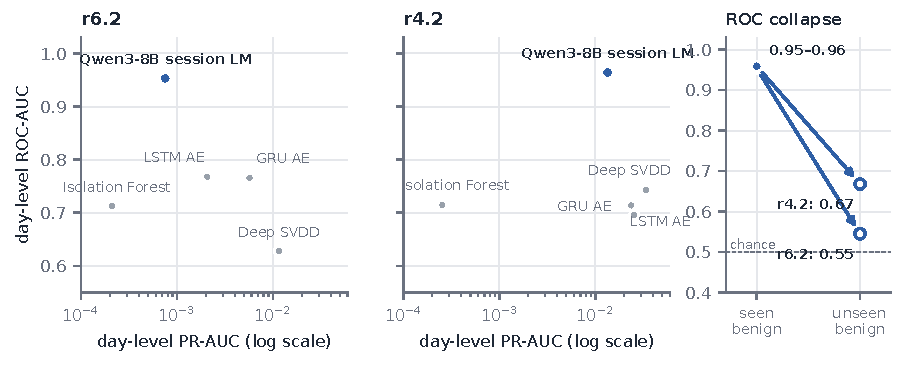
\includegraphics[width=\textwidth]{figures/detector_dissociation.pdf}
\caption{Score-level results. Left and center panels: ranking quality
(vertical axis) and average precision, the area under the precision--recall curve (horizontal axis, logarithmic scale) for
the language-model detector (blue) and four standard anomaly-detection
methods on the two benchmarks; the language model attains the highest
ranking quality under the standard protocol. Right panel: the same
language-model ranking quality when malicious users are compared only
against benign users never seen during training. The apparent advantage
largely disappears (from $0.95$ to $0.55$ on r6.2 and from $0.96$ to
$0.67$ on r4.2), and the dashed line marks chance level.}
\label{fig:collapse}
\end{figure}

\subsection{A real-data test with real personality scores}
\label{sec:plain-twos}

The CERT data are simulated, including the personality scores, so we
repeated the entire pipeline on TWOS, a dataset collected from
twenty-four real users over one week, during which some users, by
design of the underlying study, temporarily took over other users'
sessions. Each real user completed a standard fifty-item Big Five
personality questionnaire, so the serialized days contain genuine
psychometric information. In this dataset half of the users experience
an attack, so profile information is a far weaker separator than in
CERT r6.2, and our account predicts that the detector should rely on
behavior. That is what the analysis finds: the selected features place
essentially all of their mass on the behavioral lines, under two
independent training runs. Decisively, the evaluation compares each
user's attacked windows with that same user's normal windows, so static
identity and personality information is held fixed and cannot explain
the observed separation (average within-user AUC $0.78$ over the $16$ users with attacked windows).

\subsection{A second real-data test, with no profile at all}
\label{sec:plain-lanl}

TWOS still contains a profile line, albeit a real one. To remove profile
information entirely we turned to a corporate login log released by Los
Alamos National Laboratory in 2015: fifty-eight days of authentication
events from a real enterprise ($12{,}425$ users, about a billion events),
during which a security ``red team'' carried out $749$ documented
intrusions using stolen credentials. Each event records only who logged
on, from which computer, to which computer, by what mechanism, and whether
it succeeded; there is no personality line and no organizational header.
We grouped each user's events into windows of thirty-two consecutive
events, called a window malicious if it contained a red-team event,
adapted the smaller three-billion-parameter sibling of our model to
benign windows only, and scored held-out windows exactly as before. Users
were divided into five groups; the model was adapted on four and the
fifth was held out, so ranking quality can be reported separately for
\emph{seen} users (in the adaptation groups) and \emph{unseen} users (the
held-out group). Because identity now sits in two fields, we trained four
versions of the detector on four versions of the text: the full line; the
user name hidden; the computer names hidden; and the user names scrambled,
each user being given another user's name throughout.

\begin{center}
\begin{tabular}{lcc}
\toprule
Identity fields in the text & Seen-user AUC & Unseen-user AUC \\
\midrule
full                  & $0.949$ & $0.497$ \\
user name hidden      & $0.944$ & $0.518$ \\
computer names hidden & $0.877$ & $\mathbf{0.627}$ \\
user names scrambled  & $0.947$ & $0.488$ \\
\bottomrule
\end{tabular}
\end{center}

The pattern of the CERT experiments returns in a dataset that has no
profile text at all. Every version ranks seen users well and unseen users far
worse: at chance, except when the computer names are hidden. Hiding or
scrambling the user name changes little (at most $0.02$ on unseen users;
scrambling with a fixed permutation relabels a user rather than removing the
label), so the shortcut is not mainly the user name. Hiding the computer
names costs some seen-user quality and buys unseen-user quality, the
trade-off produced by CERT's profile lines, although the fraction of alerts
that would be correct on unseen users stays at the base rate in every
version (average precision about $0.013$ at a prevalence of $0.65$ percent),
so the gain is in ranking, not in usable alerts. Computer names are
associated with users without being fixed per user: a typical user's most
frequent computer accounts for about half of that user's events (median $54$
percent), and only $7$ percent of users issue at least $80$ percent of their
events from one computer. The computer name is therefore a partial proxy for
identity that may also encode which resources a user reaches, so its analogy
with CERT's fixed personality line is qualitative. A gap between seen and
unseen users remains after the computer names are hidden ($0.88$ versus
$0.63$), which may reflect genuine differences between people's behavior,
residual identity cues, or both. Two cautions apply: each of these four
detectors was trained once, and the intrusions are staged credential theft
rather than the insider scenarios of CERT, so the numbers replicate the
mechanism rather than benchmark a product.

\subsection{Retraining without the profile: is the profile the cause?}
\label{sec:plain-factorial}

Everything so far shows that a detector trained \emph{with} the profile
present relies on it. A skeptic can still ask whether the profile is the
cause of the failure on unseen users or merely something the detector
happens to notice. The direct test is a controlled experiment: train
several detectors that are identical in every respect except the profile
block, and compare them on the same unseen users. We trained four such
detectors on CERT r6.2, at both the eight-billion-parameter model of the
main paper and its three-billion-parameter sibling: (i) the full text;
(ii) the personality line removed; (iii) both profile lines removed;
(iv) the profiles scrambled, meaning that every user is given another
user's profile throughout, so the text keeps the same form, the same statistics, and the same
constancy within each user, but the profile no longer describes its owner.

For each detector we used the strictest evaluation available. Each of the
four malicious users in r6.2 is held out in turn and ranked against all $406$ benign users of this pool that were never used in
training (the protocol's cap of $800$ exceeds the pool); a user's score is the
largest of its daily scores; the AUC is averaged over the four held-out
users. Uncertainty comes from resampling the malicious users ten thousand
times and recomputing everything, which yields an interval for each
number and, because the same users are resampled for every detector, a
paired interval for the difference between two detectors. With only four
malicious users these intervals are descriptive: they say how much the
average depends on which users were held out, for these particular trained
detectors, and nothing about how a retrained detector would differ.

\begin{center}
\begin{tabular}{lcc}
\toprule
Text the detector was trained on & 3B model & 8B model \\
\midrule
full                       & $0.926$ & $0.532$ \\
personality line removed   & $0.903$ & $\mathbf{0.906}$ \\
both profile lines removed & $0.956$ & $\mathbf{0.903}$ \\
profiles scrambled         & $0.656$ & $0.485$ \\
\midrule
removal effect (both removed $-$ full) & $+0.03$ [$-0.07$, $+0.14$] & $\mathbf{+0.37}$ [$+0.07$, $+0.69$] \\
\bottomrule
\end{tabular}
\end{center}

Read the 8B column first, since that is the model of the main paper. With
the profile present, the detector ranks unseen users at chance ($0.532$).
With the profile removed it ranks them at $0.903$. The difference, $+0.37$, has a resampling interval that excludes zero: for
this detector the profile is not merely noticed; its presence in the text
used for training and scoring \emph{causes} the failure on unseen users, and
removing it repairs the detector. (Three of the four users improve, by
$+0.29$ to $+0.82$; the fourth, already caught, slips by $0.05$.) Removing the personality line alone repairs it just
as well ($0.906$), so that line is the carrier.

Now read the 3B column. The smaller model does not fail in the first
place: with the profile present it already ranks unseen users at $0.926$,
and removing the profile changes little ($+0.03$, an interval that includes
zero). Yet when we open the small model by the method of
Section~\ref{sec:plain-inside}, its selected features are just as
profile-bound as the large model's. The small model has \emph{noticed} the
profile without being measurably harmed by it. It is tempting to read this
as a size effect, and it is consistent with the capacity explanation offered
later, but the two models differ in more than size (they come from different
model generations with different pre-training), each was trained once, and a
difference that is not statistically detectable is not a demonstrated
absence. What the experiment establishes is the causal role of the profile
in the large model we audited.

Looking user by user makes the mechanism concrete. The large model's
failure is not spread evenly: one of the four malicious users is still
caught, two are ranked at chance, and one is ranked among the \emph{least}
suspicious of the $407$ users compared, worse than a coin flip. That last
user is the one whose five personality scores most closely resemble those of
many benign training users ($12$ such users nearby), and the user still
caught has few such neighbours ($3$); the ordering is only approximate,
since the user with no close neighbours at all is one of the two ranked at
chance. A large model trained on normal users learns that familiar
personality scores mean ``normal,'' and a malicious user who happens to have
ordinary scores can be waved through. With the profile removed, all four
users are ranked in the top fifth of the $407$ (positions $10$ to $75$ for
the large model, $4$ to $64$ for the small one); the user who was already
caught slips slightly, the other three rise.
Scrambling the profiles never helps: a fixed description that belongs to
someone else is at best useless and at worst misleading, even though it is
just as constant within each user as the true one. One further
observation deserves recording. When we open the scrambled-profile model,
its selected features are still profile-bound, exactly as in the
honest-profile model, even though its ranking of unseen users has
collapsed. Where a model \emph{looks} and what \emph{helps} it are
different things, which is why this paper tests features by intervening
on them rather than by attribution alone.

\subsection{Where the shortcut comes from}

One might suspect that the r6.2 data simply force any statistical method
to use profile information. This is testable. We trained three classical
anomaly detectors (an isolation forest, a one-class support vector
machine, and a principal-component reconstruction method; their details
do not matter here) on the same days, represented as ordinary numeric
feature vectors that \emph{include} the profile variables. All three
essentially ignore the profile variables: those variables receive about
four to seven percent of the total importance, no profile variable
appears among any method's top five, and deleting the profile variables
does not hurt their performance.

The shortcut is therefore not an inevitable consequence of the
available profile information: we do not observe comparable profile
reliance in the three classical detectors. An explanation consistent
with this evidence lies in the training objective. For a
likelihood-based sequence model, the per-user-constant profile tokens
are the most predictable part of every training sequence, so learning
them yields a large and cheap reduction of the training loss. In
a plain feature-vector representation, the same information is twelve
columns among two hundred forty-two, with no comparable incentive
attached. Our summary of the whole phenomenon is a two-factor statement:
the population structure of a dataset determines \emph{when} an
identity shortcut is available, and the training objective together with
the data representation determines \emph{which} detectors take it. The retraining experiment adds that, in the large model we audited, the
profile's presence in the text causes the failure rather than merely
accompanying it, and the login-log experiment adds that the shortcut lands
on whichever field reveals identity, even a field that is only associated
with a user rather than fixed: the computer name there, the personality
line here.

\section{Why this matters}

Three conclusions carry beyond these particular datasets and this
particular model.

First, for anomaly detectors intended to detect behavior, ranking
quality alone is not evidence of success. A detector should be evaluated
with the unfamiliarity confound removed, by comparing malicious
observations only against normal observations from equally unseen
users, and, where possible, by within-user comparisons.

Second, including static descriptors of people (role, department,
personality measures) in a detector's input is not harmless. In the
likelihood-based detector it created the shortcut, and even where the
detector was behavioral it degraded performance. Retraining the large
model with the profile removed repairs its ranking of unseen users from
chance to about $0.90$.

Third, the question ``what does this detector actually detect?'' can be
answered, not merely asked. The chain presented here, namely
differences of internal states, a sparse dictionary approximation,
selection of score-relevant directions, and attribution of those
directions to input content, turns the question into a measurable
quantity. In the full paper this chain is supported by causal
intervention experiments and an extensive robustness program, and it is
that combination, rather than any single number, that justifies the
conclusions summarized here.

\end{document}
